\documentclass[default]{beamer}
\setbeamertemplate{navigation symbols}{}

\usetheme{Frankfurt}
%\useoutertheme{infolines}
\usecolortheme{beaver}

\usepackage[utf8]{inputenc}					% Выбор языка и кодировки
\usepackage[english, russian]{babel}	% Языки: русский, английский
\usepackage{csquotes}
\usepackage{tikz}
\usetikzlibrary{arrows,shapes,calc}
\usepackage{animate}
\usepackage{fp}
\usepackage{textpos}

\usepackage[
	language=auto,
	autolang=other,
	backend=biber,
	style=authortitle,
	sorting=ydnt,
	maxbibnames=5
]{biblatex}
\addbibresource{strl_cai16.bib}
				
\DeclareSourcemap{
	\maps[datatype=bibtex, overwrite]{
		\map{
			\step[fieldset=langid, fieldvalue=english]
			\step[fieldset=doi, null]
			\step[fieldset=issn, null]
			\step[fieldset=isbn, null]
			\step[fieldset=url, null]
			\step[fieldsource=language, fieldset=langid, origfieldval]
		}
	}
}
\DeclareBibliographyDriver{std}{%
	\usebibmacro{bibindex}%
	\usebibmacro{begentry}%
	\usebibmacro{author/editor+others/translator+others}%
	\setunit{\labelnamepunct}\newblock
	\usebibmacro{title}%
	\newunit\newblock
	\usebibmacro{maintitle+booktitle}
	\newunit\newblock
	\usebibmacro{journal}%
	\newunit\newblock
	\usebibmacro{date}%
	\newunit\newblock
	\usebibmacro{finentry}
}
\DeclareBibliographyAlias{article}{std}
\DeclareBibliographyAlias{book}{std}
\DeclareBibliographyAlias{inproceedings}{std}
\DeclareBibliographyAlias{incollection}{std}

\graphicspath{{../../images/}} 			% Пути к изображениям

\makeatletter
\setbeamertemplate{footline}
{
	\leavevmode%
	\hbox{%
		\begin{beamercolorbox}[wd=.333333\paperwidth,ht=2.25ex,dp=1ex,center]{author
				in head/foot}%
			\usebeamerfont{author in
				head/foot}\insertshortauthor~~\beamer@ifempty{\insertshortinstitute}{}{(\insertshortinstitute)}
		\end{beamercolorbox}%
		\begin{beamercolorbox}[wd=.333333\paperwidth,ht=2.25ex,dp=1ex,center]{title in
				head/foot}%
			\usebeamerfont{title in head/foot}\insertshorttitle
		\end{beamercolorbox}%
		\begin{beamercolorbox}[wd=.333333\paperwidth,ht=2.25ex,dp=1ex,right]{date in
				head/foot}%
			\usebeamerfont{date in head/foot}\insertshortdate{}\hspace*{2em}
			\insertframenumber{}\hspace*{2ex} 
		\end{beamercolorbox}
	}%
	\vskip0pt%
}

\renewcommand*{\bibfont}{\tiny}
\setlength\bibitemsep{-5pt}

\begin{document}
	
	\title[Направления и перспективы ИИ]{Основные направления и перспективы работ в области искусственного интеллекта}
	\author[Г.С. Осипов]{\textbf{Г.С. Осипов}\\ECCAI EurAI Fellow}
	\institute[ФИЦ ИУ РАН]{Федеральный исследовательский центр <<Информатика и управление>>\\Российской академии наук}
	\date{14 ноября 2016 -- Skolkovo.AI} 
	
	{
	\setbeamertemplate{headline}{}
	\begin{frame}
		
		\titlepage
		\centering
		\href{mailto:gos@isa.ru}{gos@isa.ru}
		
		
\includegraphics[width=100pt]{misc/logos/ras.png} \hspace{10pt}
		
\includegraphics[width=80pt]{misc/logos/frccsc.png} \hspace{10pt}
		
\includegraphics[width=40pt]{misc/logos/raai.png}
	\end{frame}
	}	

	\section{Немного истории}
	\subsection{1.1}
	\begin{frame}
		\frametitle{Как это случилось}

		\begin{itemize}
			\item \textbf{1954 г.} --- аналитики \textit{Рэнд Корпорейшн}, \textit{А. Ньюэлл}, \textit{Дж. Шоу} и \textit{Г.Саймон}  решили написать программу игры в шахматы. В этой затее им вызвались помочь \textit{А. Тьюринг} и \textit{К. Шеннон}, а также группа голландских психологов.
			\item \textbf{1957 г.} --- программа для игры в шахматы (NSS) таки была написана. В основе работы NSS лежали эвристики --- правила выбора в отсутствие теоретических оснований.
		\end{itemize}
	\end{frame}
	\subsection{1.2}
	\begin{frame}
	\frametitle{Что произошло дальше}
	
		\begin{itemize}
			\item \textbf{1960 г.}  --- GPS (<<универсальный решатель задач>>): вычисление неопределенных интегралов, головоломки и  некоторые другие задачи.  Программы автоматического доказательства теорем из планиметрии, решения алгебраических задач. 
			\item \textbf{1960 г.} --- возникновение \textbf{эвристического программирования}. 
			\item \textbf{1963 г.} --- \textit{Джон Маккарти} --- ЛИСП. \textbf{Возникновение функционального программирования}.
		\end{itemize}
	\end{frame}
	\subsection{1.3}
	\begin{frame}
		\frametitle{Поиск непереборных методов решения задач}
		
		\begin{itemize}
			\item \textbf{1964 г.} --- \textit{В.Н. Пушкин} и \textit{Д.А. Поспелов}  --- модельная гипотеза мышления versus лабиринтной; методы решения переборных задач человеком. 
			\item \textbf{1964 г.} --- \textit{С.Ю. Маслов} --- метод автоматического поиска доказательства теорем в исчислении предикатов (обратный метод).
			\item \textbf{1965 г.} --- \textit{Дж.А. Робинсон} --- метод автоматического поиска доказательства теорем в исчислении предикатов (метод резолюций).
			\item \textbf{1968 г.} --- возникновение \textbf{логического программирования}.
			\item \textbf{1971 г.} --- \textit{А. Колменрауэр} --- \textbf{язык Пролог}.
			
		\end{itemize}
	\end{frame}

	\subsection{1.4}
	\begin{frame}
		\frametitle{Современный ИИ}
		\Large
		\begin{itemize}
			\item \textbf{Середина 70-х гг.} --- качественный скачок в работах по искусственному интеллекту.
			\item Появление  первых прикладных систем, использующих знания для решения различных всё более сложных задач.
		\end{itemize}
	\end{frame}

	\section{Организация ИИ}
	\subsection{2.1}
	\begin{frame}
		\frametitle{Искусственный интеллект --- организационная структура}
		
		Европейская ассоциация искусственного интеллекта  (EurAI), возглавляемая координационным 	комитетом (ECCAI), который, в свою очередь, состоит из выборных членов (members) и постоянных (fellows).
		
		\begin{itemize}
			\item Каждые два года (по четным годам) проводится Европейская конференция по искусственному интеллекту (ECAI).
			\item ECAI 2016 состоялась в Гааге. Обычно в этих конференциях принимает участие от 500 до 700 исследователей из разных (не только европейских) стран.
		\end{itemize}
	\end{frame}

	\subsection{2.2}
	\begin{frame}
		\frametitle{Конференции}
		
		\begin{itemize}
			\item Наша ассоциация принимала участие \textbf{в организации} ECAI 1996, ECAI 1998, ECAI 2000, ECAI 2006 и ряде иных общеевропейских мероприятий.
			\item Ежегодно проходит  Международная объединённая конференция по искусственному интеллекту (IJCAI), организуемая совместно Европейской и Американской ассоциациями искусственного интеллекта. В этом году она проходила в Нью-Йорке. В ней приняли участие два моих ученика.
			\item Ежегодно в разных странах проходит JCKBSE, впервые организованная РАИИ; и по сей день мы принимаем участие в её организации и научной программе.  
		\end{itemize}
	\end{frame}

	\subsection{2.3}
	\begin{frame}
		\frametitle{Российская ассоциация искусственного интеллекта}
		
		\begin{itemize}
			\item Общероссийская общественная организация --- 261 индивидуальный член, 45 региональных отделений.
			\item По четным годам (совместно с рядом академических организаций и вузов) проводится Национальная конференция по искусственному интеллекту. В этом году --- 15я Национальная конференция, Смоленск, 131 доклад, около 200 участников.
		\end{itemize}
	\end{frame}

	\subsection{2.4}
	\begin{frame}
		\frametitle{Искусственный интеллект и принятие решений}
		\Large
		\begin{itemize}
			\item Журнал с таким названием издаётся РАН совместно с РАИИ.
			\item 6 номеров в год: 4 на русском и два на английском (Шпрингер).
			\item Сайт журнала \href{aidt.ru}{aidt.ru}.
		\end{itemize}
	\end{frame}

	\section{Направления ИИ}
	\subsection{3.1}
	\begin{frame}
		\frametitle{Основные направления ИИ}
		\centering
		\footnotesize
		\makebox[0.8\textwidth][c]{
			\begin{tikzpicture}
				\node[ellipse, minimum width = 100, minimum height = 50, fill=blue!20, align=center] (d1) {Искусственный\\интеллект};
				
				\node[rounded corners=5pt,draw,color=blue!20, very thick,text=black] (d2) at (-4,2) {
					\begin{minipage}[c][33pt]{100pt}
						\centering
						\textbf{Приобретение знаний, анализ данных и порождение гипотез}
					\end{minipage}
				};
				\node[rounded corners=5pt,draw,color=blue!20, very thick,text=black] (d3) at (-4,0.5) {
					\begin{minipage}[c][20pt]{80pt}
					\centering
					\textbf{Моделирование рассуждений}
					\end{minipage}
				};
	
				\node[rounded corners=5pt,draw,color=blue!20, very thick,text=black] (d4) at (-4,-0.7) {
					\begin{minipage}[c][20pt]{80pt}
					\centering
					\textbf{Многоагентные системы}
					\end{minipage}
				};
			
				\node[rounded corners=5pt,draw,color=blue!20, very thick,text=black] (d5) at (-4,-2.3) {
					\begin{minipage}[c][43pt]{110pt}
					\centering
					\textbf{Обработка естественного языка, пользовательский интерфейс и модели пользователя}
					\end{minipage}
				};
			
			
				\node[rounded corners=5pt,draw,color=blue!20, very thick,text=black] (d6) at (4,2) {
					\begin{minipage}[c][33pt]{120pt}
					\centering
					\textbf{Динамические интеллектуальные системы и планирование поведения}
					\end{minipage}
				};
				\node[rounded corners=5pt,draw,color=blue!20, very thick,text=black] (d7) at (4,0.5) {
					\begin{minipage}[c][20pt]{80pt}
					\centering
					\textbf{Представление знаний}
					\end{minipage}
				};
				
				\node[rounded corners=5pt,draw,color=blue!20, very thick,text=black] (d8) at (4,-0.7) {
					\begin{minipage}[c][20pt]{100pt}
					\centering
					\textbf{Нечеткие модели и мягкие вычисления}
					\end{minipage}
				};
				
				\node[rounded corners=5pt,draw,color=blue!20, very thick,text=black] (d9) at (4,-2.3) {
					\begin{minipage}[t][20pt]{110pt}
					\centering
					\textbf{Инструментальные средства и технологии}
					\end{minipage}
				};
				
				\draw[->,rounded corners=10pt, very thick, blue!20](d1)[xshift=-10] |- (d2.east);
				\draw[->,rounded corners=10pt, very thick, blue!20](d1)[xshift=10] |- (d6.west);
				
				\draw[->,rounded corners=10pt, very thick, blue!20](d1)[xshift=-10] |- (d5.east);
				\draw[->,rounded corners=10pt, very thick, blue!20](d1)[xshift=10] |- (d9.west);
				
				\draw[->,rounded corners=10pt, very thick, blue!20](d1) |- (d3.east);
				\draw[->,rounded corners=10pt, very thick, blue!20](d1) |- (d7.west);
				
				\draw[->,rounded corners=10pt, very thick, blue!20](d1.south west) |- (d8.west);
				\draw[->,rounded corners=10pt, very thick, blue!20](d1.south east) |- (d4.east);
			\end{tikzpicture}
		}
	\end{frame}

	\subsection{3.2}
	\begin{frame}
		\frametitle{Приобретение знаний, анализ данных и автоматическое порождение гипотез}
		
		\textbf{Цель}: создание методологий, технологий и программных средств обнаружения и переноса компетентности   в базы знаний.
		\par\medskip
		\centering
		\tikz[baseline]{
			\small
			\node[fill=yellow, rounded corners=5pt, minimum width=300, minimum height = 150] (k1) {
				\begin{minipage}[t][150pt]{300pt}
					\centering
					\textbf{Методы приобретения знаний:}
				\end{minipage}
				
			};
			
			\node[rounded corners=5pt, minimum width=280, minimum height = 50, text width= 250, text centered,fill=white] (k2) at (0, 0.85) {
				\begin{minipage}[t][60pt]{250pt}
					\centering
					\textbf{Машинное обучение и обучение по примерам} (методы построения деревьев решений,  индуктивные методы построения правил;  статистические методы, в частности, Байесовские  сети; метод ближайших соседей, искусственные нейронные сети)
				\end{minipage}
				
			};
		
			\node[rounded corners=5pt, minimum width=280, minimum height = 10, text width= 250, text centered,fill=white] (k2) at (0,-0.9) {
				\begin{minipage}[t][10pt]{250pt}
					\centering
					\textbf{Приобретение знаний из текстов}
				\end{minipage}
				
			};
		
			\node[rounded corners=5pt, minimum width=280, minimum height = 20, text width= 250, text centered,fill=white] (k2) at (0, -2) {
				\begin{minipage}[t][20pt]{250pt}
					\centering
					\textbf{Прямые методы приобретения знаний (автоматизированный диалог с экспертами)}
				\end{minipage}
				
			};
		}
	\end{frame}

	\subsection{3.3}
	\begin{frame}
		\frametitle{Представление знаний}
		
		\textbf{Предмет}:  разработка языков и программных средств   для описания экспертных и эмпирических знаний. 
		\par\medskip
		\textbf{Содержание}:
		\begin{itemize}
			\item семантические сети, системы фреймов, системы правил (продукционные системы) и их гибриды;
			\item логики пространства и времени;
			\item онтологии – способ обмена знаниями;
			\item дескриптивные логики (теория баз знаний и онтологий).
		\end{itemize}
	\end{frame}

	\subsection{3.4}
	\begin{frame}
		\frametitle{Автоматизация  рассуждений}
		
		Методы индукции, абдукции и аналогии, аргументации, рассуждения на основе прецедентов, на основе ограничений, рассуждения о действиях и изменениях, рассуждения с неопределенностью, немонотонные рассуждения.
		\par\medskip
		\tikz[baseline]{
			\node[fill=blue!20, rounded corners=5pt, anchor=base] (t1) {\textbf{Немонотонные рассуждения}};
		}
		связаны с поиском эмпирических зависимостей в данных, обучением по примерам и рассуждениями в эмпирических  теориях. Выделились в самостоятельный раздел логики.
		\par\medskip
		\tikz[baseline]{
			\node[fill=blue!20, rounded corners=5pt, anchor=base] (t2) {\textbf{Рассуждения о действиях}};
		}
		исследуют связь  действий и эффектов действий (результатов действий).
		\par\medskip
		\tikz[baseline]{
			\node[fill=blue!20, rounded corners=5pt, anchor=base] (t3) {\textbf{Рассуждения с неопределенностью}};
		}
		--- использование  Байесовского  формализма в моделях рассуждений. 
		
	\end{frame}

	\subsection{3.5}
	\begin{frame}
		\frametitle{Многоагентные системы}
		
		Изучаются интеллектуальные программные агенты, их коалиции и поведение.
		
		\par\medskip
		\textbf{Интеллектуальный программный  агент} --- программная система, обладающая автономностью, социальными чертами, реактивностью и активностью.
		
		\par\medskip
		\textbf{Основные проблемы}: коммуникация интеллектуальных агентов, разработка языков для этой цели, координация поведения  агентов, распределение ролей в коалициях агентов, коллективное поведение агентов.
	\end{frame}

	\subsection{3.6}
	\begin{frame}
		\frametitle{Учиться лучше вместе}
		\Large 
		\textbf{Экспериментальным результатом исследования обучения агентов явилось то, что группа агентов лучше обучается решению сложных задач, чем индивидуально на тех же самых примерах.} 
		
	\end{frame}

	\subsection{3.7}
	\begin{frame}
		\frametitle{Роботы и автономные системы}
		\Large
		\begin{itemize}
			\item Диалоговое взаимодействие коалиций мобильных роботов.
			\item Интерпретация команд, поступающих от человека.
			
			\item Качественные логики пространства-времени.
			
			\item Рассуждения, основанные на оценках.
			
		\end{itemize}
		
	\end{frame}

	\subsection{3.8}
	\begin{frame}
		\frametitle{Интеллектуальные динамические системы и автоматическое планирование поведения}
		\Large
		
		\textbf{Результат интеграции} методов искусственного интеллекта с теорией динамических систем:
		\begin{itemize}
			\item планирование,
			\item моделирование,
			\item управление.
		\end{itemize}
		
	\end{frame}

	%\subsection{3.9}
	\begin{frame}
		\frametitle{Обработка естественного языка, интерфейс и модели пользователя}
		\begin{itemize}
			\small
			\item Семантический поиск в больших массивах текстов:
			\begin{itemize}
				\footnotesize
				\item поиск документов (в полнотекстовой БД, в локальных и глобальных телекоммуникационных сетях);
				\item извлечение данных из текстов;
				извлечение знаний из текстов.
			\end{itemize}
			
			\item Обработка текстов: сегментация, классификация, кластеризация, аннотирование или реферирование текстов. Перевод. 
			\item Диалоговые системы: 
			\begin{itemize}
				\footnotesize
				\item интеллектуальные вопросно-ответные системы; 
				\item системы общения конечных пользователей с БД, предоставляющие  различные услуги (выполнение банковских операций по телефону, заказ товаров по каталогам); 
				\item голосовое управление техникой, кооперативное решение проблем (человек плюс интеллектуальная система).
			\end{itemize}
			
			\item Автоматическое обучение анализу текстов.
			
		\end{itemize}
		
	\end{frame}

	\subsection{3.10}
	\begin{frame}
		\frametitle{Нечеткие модели и мягкие вычисления}
		
		\Large 
		\begin{itemize}
			\item Нечеткие схемы вывода по аналогии;
			\item теория нечетких мер; 
			\item модели геометрических объектов;
			\item алгоритмы эволюционного моделирования с динамическими параметрами (например, время жизни и размер популяции);
			\item методы решения оптимизационных задач с использованием технологий генетического поиска, гомеостатических и синергетических принципов и элементов самоорганизации. 
		\end{itemize}
		
	\end{frame}

	\subsection{3.11}
	\begin{frame}
		\frametitle{Вклад ИИ в другие  науки}
		
		Развитие ИИ привело к \textbf{возникновению самостоятельных областей}:
		\begin{itemize}
			\item эвристическое программирование,
			\item функциональное программирование,
			\item логическое программирование,
			\item объектно-ориентированное программирование,
			\item теория немонотонных рассуждений и немонотонные логики,
			\item инженерия знаний,
			\item технология программирования, основанная на знаниях,
			\item прикладная семиотика.
		\end{itemize}
		
		В \textbf{инженерном направлении}:
		\begin{itemize}
			\item экспертные системы.
		\end{itemize}
	\end{frame}

	\section{Перспективы ИИ}
	\subsection{4.1}
	\begin{frame}
		\frametitle{Перспективные направления ИИ}
		
		\begin{itemize}
			\item \textbf{Рассуждения, основанные на прецедентах}.
			\item \textbf{Рассуждения о пространстве} --- возрастающее значение для автономных мобильных устройств, анализа изображений (в частности, аэрофотоснимков), синтеза текстовых описаний по изображениям.
			\item \textbf{Методы машинного обучения и автоматического формирования гипотез} --- решение практических задач: от обнаружения  закономерностей в данных до повышения степени адаптивности различных технических устройств.
			\item Подходы, основанные на \textbf{технологии интеллектуальных агентов} перспективны при разработке больших программных систем.
			
		\end{itemize}
		
	\end{frame}

	\subsection{4.2}
	\begin{frame}
		\frametitle{Перспективные направления ИИ}
		
		\begin{itemize}
			\item \textbf{Влияние идей и методов ИИ на машинный анализ текстов на естественном языке} --- коснется  семантического анализа и методов синтаксического анализа --- в этой области оно проявится в учете модели мира и использовании знаний о предметной области  для уменьшения переборов  на более ранних стадиях анализа.
			\item \textbf{Понимание текста}.
			\item \textbf{Автоматическое планирование и управление поведением}. Область применения  - от бытовой  техники до беспилотных аппаратов для исследования глубокого космоса.
		\end{itemize}
		
	\end{frame}

	\subsection{4.3}
	\begin{frame}
		\frametitle{Перспективные направления ИИ}
		
		\begin{itemize}
			\item Управление подготовкой к пуску ракет космического	назначения.
			\item Автономные мобильные средства ведения боевых операций.
			\item Моделирование бизнес --- процессов на основе систем бизнес-правил.
			\item Банковские системы, например,  анализ транзакций с целью выявления сомнительных операций и  мошенничества или обнаружение так называемого layering (лээринга) --- действия покупателя пакета акций, направленные на снижение цены этих акций посредством создания фиктивного предложения больших пакетов этих акций;
			\item и ряд других приложений в этой сфере.
			
		\end{itemize}
		
	\end{frame}

	\subsection{4.4}
	\begin{frame}
		\frametitle{Проблемы}
		
		\begin{itemize}
			\item Переход от моделирования структурной организации к моделированию ментальных представлений, в частности, когнитивных функций, иначе говоря,от искусственного интеллекта --- к искусственному сознанию.
			\item Автоматическое (или полуавтоматическое) формирование интеллектуальными агентами модели мира, включая зрительные и слуховые образы предметов и их назначение.

		\end{itemize}
		
	\end{frame}

	\section{Результаты РААИ}
	\subsection{5.1}
	\begin{frame}
		\frametitle{Некоторые результаты коллективов-членов РААИ}
		
		\begin{itemize}
			\item Получены результаты  сравнительного анализа систем аргументации. Предложено использовать механизмы аргументации для обнаружения и разрешения внутренних противоречий в базе знаний ИСППР. 
			\item Введены степени обоснования, что значительно расширяет класс задач, решаемых с помощью системы аргументации, а также использует системы аргументации как мощное средство для обнаружения и разрешения конфликтов в базах знаний. \textbf{(МЭИ)} 
		\end{itemize}
	\end{frame}

	\subsection{5.2}
	\begin{frame}
		\frametitle{ИПУ РАН}
		\Large
		\begin{itemize}
			\item Разработана программная система <<Канва>> для поддержки принятия решений в слабоструктурированных ситуациях. 
			
			\item Разработан комплекс моделей поддержки принятия решений в конфликтных ситуациях с использованием когнитивных карт. 
			
		\end{itemize}
	\end{frame}
	
	\subsection{5.3}
	\begin{frame}
		\frametitle{ГосНИИАС}
		\Large
		\begin{itemize}
			\item Для модели летательного аппарата <<Этап>>	разработана теория бортовых 	интеллектуальных систем тактического уровня (БИС-Т/У), решающих задачи оперативного целеполагания и конструирования способа достижения оперативно назначенной цели.
			\item Для пилотируемых летательных аппаратов эти системы создаются в форме бортовых оперативно советующих экспертных систем (БОСЭС-целеполагание и БОСЭС-типовой ситуации полета). 
		\end{itemize}
	\end{frame}

	\subsection{5.4}
	\begin{frame}
		\frametitle{НИЦ <<Курчатовский институт>>}

		\begin{itemize}
			\item Созданы роботы, архитектура системы управления которых включает эмоциональную компоненту. Поведение такого робота определяется комплексом эмоций, испытываемым им в зависимости от текущих потребностей и оценкой возможности их (потребностей) удовлетворения. Развитием этого направления стало создание механизма темперамента робота. В зависимости от задаваемых параметров, можно определить поведение робота как холерическое, сангвиническое, флегматическое и меланхолическое. 
			\item Определены условия, при которых та или иная организация темперамента поведения является наиболее выгодной для робота. 
			
		\end{itemize}
	\end{frame}
	
	\subsection{5.5}
	\begin{frame}
		\frametitle{ИПМ РАН}
		\Large
		\begin{itemize}
			\item Разработаны технологии поддержки интеллектуальных роботов-манипуляторов, способных автоматически принимать решения непосредственно во время работы. Технологии позволяют управлять поведением робота-манипулятора МанГо во время логической игры; рассмотрены настольные игры типа Го или Гомоrу. 
		\end{itemize}
	\end{frame}

	\begin{frame}
		\frametitle{ИПМ РАН}
		
		\begin{itemize}
			\item Разработана подсистема зрения робоавтомобиля АвтоНИВА. Система зрения работает с цветными телевизионными изображениями. Подсистема основана на новом, специальном сжатом описании каждого кадра, которое позволяет решать задачи нахождения и распознавания объектов в реальном времени, минимизируя обращения к исходному массиву изображения на стандартном персональном компьютере. Описана система выделения препятствий на пути движения автомобиля по дальномерным данным. 
		\end{itemize}
	\end{frame}

	\subsection{5.6}
	\begin{frame}
		\frametitle{ФИЦ ИУ РАН}
		\Large
		\begin{itemize}
			\item Создана семантическая поисковая машина нового поколения EXACTUS.  Машина работает с запросами на естественном языке.
			\item Неоднократно занимала первые места по релевантности поиска на соревнованиях поисковых 	машин \href{www.exactus.ru}{www.exactus.ru}.
		\end{itemize}
	\end{frame}
	
	\begin{frame}
		\frametitle{ФИЦ ИУ РАН}
		\Large
		\begin{itemize}
			\item Создана система прогнозирования социального стресса на основе анализа социальных медиа.
			\item Созданы системы
			\begin{itemize}
				\item EXACTUS EXPERT --- для cемантического поиска и анализа качества научных публикаций,
				\item EXACTUS PATENT --- для семантического поиска и анализа патентной информации.
			\end{itemize}
		\end{itemize}
	\end{frame}

	
	\begin{frame}
		\frametitle{ФИЦ ИУ РАН}
		\centering
		
		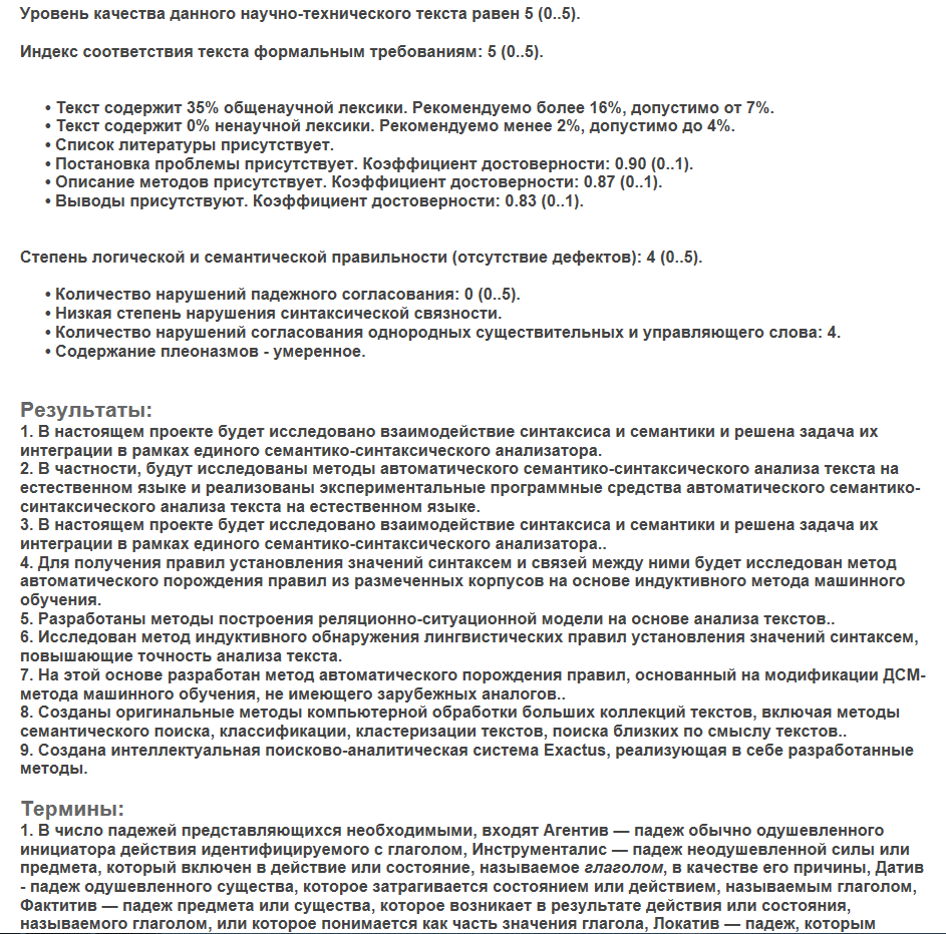
\includegraphics[width=0.75\textwidth]{misc/exactus/analytics.png}
	\end{frame}
	
	\subsection{5.7}
	\begin{frame}
		\frametitle{ФИЦ ИУ РАН}
		
		\begin{itemize}
			\item EXACTUS LIKE для обнаружения близких текстов и вычисления степени семантической близости;
			\item TEXT Appliance --- информационно-аналитическая система анализа неструктурированной информации.
			\item TEXT Appliance куплена национальным цифровым ресурсом  Руконт и используется  десятками вузов и компанией Инфра-М.
		\end{itemize}
	\end{frame}

	\section*{}
	{
	\setbeamertemplate{headline}{}
	\begin{frame}
		\centering
		\Huge
		Спасибо за внимание!
		\normalsize
		\par\bigskip
		\par\bigskip
		ФИЦ ИУ РАН
		
		\par\bigskip
		gos@isa.ru
	\end{frame}			
	}
\end{document}
	
	
